\documentclass[11pt]{article}

\usepackage[margin=1in]{geometry}
\usepackage{amsmath,amssymb,amsfonts}
\usepackage{booktabs}
\usepackage{graphicx}
\usepackage{siunitx}
\usepackage{xcolor}
\usepackage{microtype}
\usepackage[colorlinks=true,linkcolor=blue,citecolor=blue,urlcolor=blue]{hyperref}
\usepackage{caption}
\usepackage{subcaption}
\usepackage{bm}
\usepackage[version=4]{mhchem}

\newcommand{\uu}{\mathbf{u}}
\newcommand{\vv}{\mathbf{v}}
\newcommand{\R}{R}
\newcommand{\etah}{\hat{\eta}}
\newcommand{\zetah}{\hat{\zeta}}
\renewcommand{\Pr}{\mathrm{Pr}}
\newcommand{\code}[1]{\texttt{#1}}

\title{\bf A spectral Wigner--Eckart evaluation of the polyatomic\\
Boltzmann collision operator with the DSMC frozen/non-frozen\\
collision kernel and its internal-energy-modulated extension}

\author{Ren\'e Hiemstra\\
\small Simkinetic}
\date{\today}

\begin{document}
\maketitle

\begin{abstract}
We implement and validate the variable-hard-sphere (VHS) Borgnakke--Larsen collision
kernel used by the direct simulation Monte Carlo (DSMC) community
[Djordji\'c, Oblapenko, Pavi\'c-\v{C}oli\'c \& Torrilhon, \emph{Continuum Mech.\ Thermodyn.}
\textbf{35} (2023) 103--119] inside a spectral Wigner--Eckart factorization of the
polyatomic Boltzmann collision operator. The kernel is a convex combination of a
\emph{non-frozen} channel (full Borgnakke--Larsen internal-energy redistribution) and a
\emph{frozen} channel (elastic, internal-energy preserving). We show that the frozen channel
must be integrated in internal-energy space with no additional partition measure -- a subtle
point whose violation injects a spurious $\delta$-dependence into the internal heat-flux
relaxation rate. With the corrected channel the operator reproduces the Eucken Prandtl number
at the analytic anchor to machine precision ($2\times10^{-14}$) and the exact monatomic shear
sector $P_\sigma^{(0)}/P_q^{(0)}=3/2$ for all $\zeta$. An independent Monte-Carlo evaluation of
the elastic collision bracket confirms our spectral frozen Prandtl number to $3$--$4$ digits
and shows that it \emph{differs} from the paper's analytic frozen formula at $\zeta\neq0$,
i.e.\ the spectral quadrature is the more accurate of the two. Finally we implement the
internal-energy-modulated extended kernel and demonstrate that, after re-fitting the free
parameters in our (more accurate) operator, it reaches the experimental Prandtl number and the
bulk/shear viscosity ratio simultaneously -- exactly and with admissible parameters for
\ce{N2} and \ce{CO}, and exactly but essentially on the kernel-positivity boundary for the
extreme case \ce{H2}.
\end{abstract}

\tableofcontents
\medskip

% =====================================================================
\section{Introduction}
\label{sec:intro}

The Boltzmann collision operator for a polyatomic gas with a continuous internal-energy
variable governs the relaxation of the distribution function $f(\vv,I)$ towards equilibrium and
fixes the gas transport coefficients (shear viscosity $\mu$, bulk viscosity $\nu$, thermal
conductivity $\kappa$, and hence the Prandtl number $\Pr$). Evaluating this operator on a
spectral basis is expensive because the gain term is a high-dimensional integral over the
collision geometry and the internal-energy redistribution.

The \emph{Wigner--Eckart factorization} reduces this cost dramatically: rotation invariance of
the collision kernel lets the operator be written as a contraction of a sparse, geometry-only
\emph{Gaunt} angular tensor with a dense, kernel-dependent \emph{physical} tensor (here denoted
the $R$-tensor). Only the $R$-tensor depends on the collision kernel, so a new kernel model
requires changes only to its quadrature -- the angular machinery is untouched.

This report integrates the DSMC collision-kernel model of Djordji\'c \emph{et al.}
\cite{Djordjic2023} into such a spectral code. The model is the variable-hard-sphere
Borgnakke--Larsen (VHS--BL) kernel, written as a convex combination of a \emph{non-frozen}
channel (internal energy redistributed) and a \emph{frozen} channel (elastic, internal energy
preserved). We (i) derive the correct spectral treatment of the frozen channel, (ii) validate
the resulting transport coefficients against analytic anchors and against an independent
Monte-Carlo computation, finding that the spectral operator is more accurate than the paper's
analytic transport formulas at hard-potential exponents, and (iii) implement the
internal-energy-modulated extended kernel and show it reaches experimental data.

% =====================================================================
\section{The collision operator and the DSMC kernel}
\label{sec:kernel}

\subsection{Operator and Wigner--Eckart factorization}
The space-homogeneous collision operator is
\begin{equation}
Q(f,f)(\vv,I) = \int \big[f(\vv',I')f(\vv_*',I_*') - f(\vv,I)f(\vv_*,I_*)\big]\,
\mathcal{B}\; d\sigma\, dR\, dr\, d\vv_*\, dI_*,
\end{equation}
with the Borgnakke--Larsen parametrization of the post-collision state by the kinetic-energy
partition $R\in[0,1]$ and the internal-energy partition $r\in[0,1]$:
\begin{equation}
e_{\mathrm{tr}}'=R,\qquad i'=r(1-R),\qquad i_*'=(1-r)(1-R),
\end{equation}
where $i=I/E$, $i_*=I_*/E$ and $E=\tfrac12|\uu|^2+I+I_*$ is the (conserved) total energy in
code units. Expanding $f$ on the spectral basis
$\phi_{k\ell m,n}(\vv,I)=R_{k\ell}(|\vv|)Y_{\ell m}(\hat\vv)\,H_n(I)$
(associated-Laguerre $\times$ spherical-harmonic $\times$ internal-Laguerre) and using rotation
invariance, $Q$ factorizes into a sparse Gaunt tensor contracted with the dense $R$-tensor
$R[k_1k_2k_3,n_1n_2n_3,\ell]$, evaluated by sum factorization (a Fubini cascade over the
energy, kinetic-partition, internal-partition and scattering integrals).

\subsection{The DSMC convex-split kernel}
The DSMC kernel \cite[eqs.~(53)--(55)]{Djordjic2023} is
\begin{equation}
\mathcal{B}_{\mathrm{DSMC}}
= |\uu|^{\zeta}\Big[\,\omega\,K_\delta\,R^{\zeta/2}\;+\;(1-\omega)\,
\delta_{r-r'}\delta_{R-R'}\,e_{\mathrm{tr}}^{\zeta/2}\,\Big],
\label{eq:dsmc}
\end{equation}
where $\zeta=2(1-s_{\mathrm{visc}})$ is the relative-speed exponent
($s_{\mathrm{visc}}$ is the viscosity temperature exponent), $\delta$ is the number of internal
degrees of freedom ($\nu=\delta/2-1$ is the internal-Laguerre parameter), $\omega=p_{\mathrm{int}}$
is the inelastic-collision probability, and
$K_\delta=2\Gamma(\delta+\tfrac32)/[\sqrt\pi\,\Gamma(\delta/2)^2]$ is the monatomic-consistency
constant. The first term is the \emph{non-frozen} (Borgnakke--Larsen) channel; the second is the
\emph{frozen} (elastic, $I'=I$, $I_*'=I_*$, $|\uu'|=|\uu|$) channel. Because the operator is
linear in $\mathcal{B}$, the $R$-tensor is a convex sum,
$R_{\mathrm{tot}}=\omega\,K_\delta R_{\mathrm{nf}}+(1-\omega)\,C_{\mathrm{VHS}}^{f}R_{\mathrm{fr}}$.

\subsection{Spectral treatment of the two channels}
\paragraph{Non-frozen channel.}
The single separable term $K_\delta|\uu|^{\zeta}R^{\zeta/2}$ folds cleanly into the existing
quadrature: $|\uu|^\zeta\propto z^{\zeta/2}$ ($z=\tfrac12|\uu|^2$) is desingularized by the
Gauss--Laguerre$(\zeta/2)$ energy rule, while $R^{\zeta/2}$ shifts the kinetic-partition
Gauss--Jacobi weight to $\mathrm{Jacobi}(2\nu+1,\tfrac12+\tfrac\zeta2)$. The integrand is
polynomial after folding, so convergence is \emph{spectral}.

\paragraph{Frozen channel (a subtle correction).}
The frozen collision is elastic with the internal energies as spectators. The natural and
correct spectral treatment integrates the frozen channel \emph{directly in internal-energy
space} over the Gauss--Laguerre nodes $(I,I_*)$ with weights $W_I W_{I_*}$; basis
orthonormality $\int H_a H_b\,I^\nu e^{-I}\,dI=\delta_{ab}$ then carries the frozen Kronecker
structure $I'=I$. There is \emph{no} $(R,r)$-partition phase-space measure in this channel.

A tempting but incorrect alternative collapses the Dirac deltas
$\delta_{r-r'}\delta_{R-R'}$ against the Borgnakke--Larsen measure
$H_\delta(r,R)=(r(1-r))^\nu(1-R)^{2\nu+1}\sqrt R$ and leaves $H_\delta$ as an explicit weight.
Because the frozen routine already integrates over the internal energies, this double-counts a
non-polynomial, $\nu$-dependent factor and injects a spurious $\delta$-dependence into the
internal-heat-flux rate (Sec.~\ref{sec:frozenpr}). The correct frozen weight is simply
$W_I W_{I_*}\,\mathcal{B}^{f}\,\mathrm{Jac}_{\mathrm{spatial}}$.

% =====================================================================
\section{Transport coefficients}
\label{sec:transport}

Linearizing the assembled operator about equilibrium gives
$J=C(:,:,1)+C(:,1,:)$, whose blocks yield the $17$-moment production terms
\cite[eqs.~(35)--(39)]{Djordjic2023}:
the shear rate $P_\sigma^{(0)}$ (mode $\ell=2,n=0$), the bulk rate $P_\Pi^{(0)}$
(mode $\ell=0,n=1$, $\propto\omega$), and the $\ell=1$ heat-flux $2\times2$ block in the
translational mode $q=(k{=}1,n{=}0,\ell{=}1)$ and internal mode $s=(k{=}0,n{=}1,\ell{=}1)$:
$P_q^{(0)}=-J_{qq}$, $P_s^{(0)}=-J_{ss}$, $P_q^{(1)}=-\rho\,J_{qs}$, $P_s^{(1)}=-J_{sq}/\rho$,
with heat-flux moment ratio
\begin{equation}
\rho=\frac{d_q}{d_s}=\sqrt{\frac{5}{4\delta}} .
\label{eq:rho}
\end{equation}
The closed form \eqref{eq:rho} is obtained numerically to machine precision. The Prandtl number
and the bulk/shear ratio follow from \cite[eqs.~(39),(58)]{Djordjic2023}:
\begin{equation}
\Pr=\frac{5+\delta}{2}\,
\frac{2\big(P_q^{(0)}P_s^{(0)}-P_q^{(1)}P_s^{(1)}\big)}
{P_\sigma^{(0)}\big[5(P_s^{(0)}-P_s^{(1)})+\delta(P_q^{(0)}-P_q^{(1)})\big]},
\qquad
\frac{\nu}{\mu}=\frac{2\delta}{3(3+\delta)}\,\frac{P_\sigma^{(0)}}{P_\Pi^{(0)}}.
\label{eq:Pr}
\end{equation}

% =====================================================================
\section{Validation of the base DSMC kernel}
\label{sec:validation}

\subsection{Reduction, conservation, and exact anchors}
With $\zeta=0$ and $\omega=1$ the kernel is constant (Maxwell) and the operator reproduces the
$5$ collision invariants and the exact Maxwell spectrum. For all parameters the mass-conservation
row vanishes to $\sim10^{-15}$ and the linearized operator has exactly $5$ null eigenvalues for a
convex blend ($7$ for the frozen-only limit, where internal energy is separately conserved).
Two analytic anchors are met exactly:
\begin{itemize}
\item \textbf{Shear sector.} $P_\sigma^{(0)}/P_q^{(0)}=3/2$ \emph{exactly for all $\zeta$},
i.e.\ the first-Sonine monatomic Prandtl number $2/3$ -- the velocity sector is exact.
\item \textbf{Eucken anchor.} At $\zeta=0,\ \omega=0$ the frozen Prandtl number equals the
Eucken value $\Pr^{\mathrm{Euck}}=2(\delta+5)/(2\delta+15)$ to $2\times10^{-14}$ for
$\delta=2,4,5$ (the analytic identity of \cite[eq.~(41)]{Djordjic2023}).
\end{itemize}

\subsection{The frozen Prandtl number is computed more accurately than the analytic formula}
\label{sec:frozenpr}
For $\zeta\neq0$ the entire $\zeta$-dependence of the frozen Prandtl number lives in
$b\equiv P_s^{(0)}/P_q^{(0)}$ (since $P_\sigma^{(0)}/P_q^{(0)}=3/2$ is exact). We compute $b$ three
ways: (i) our spectral operator; (ii) the paper's analytic frozen formula \cite[eq.~(42)]{Djordjic2023},
\begin{equation}
\Pr^{\mathrm{Frozen}}=\frac{2(\delta+5)}{\delta\big(2+\tfrac45\zeta\big)\frac{2\delta+2\zeta+7}{2\delta+\zeta+7}+15},
\qquad
b_{\mathrm{eq42}}=\frac{3(2\delta+\zeta+7)}{(2+\tfrac45\zeta)(2\delta+2\zeta+7)};
\end{equation}
and (iii) an independent Monte-Carlo evaluation of the rigorous elastic-collision $H$-theorem
bracket, $-\langle\phi,L\phi\rangle=\tfrac14\,\mathbb{E}\big[(\phi+\phi_*-\phi'-\phi_*')^2|\uu|^\zeta\big]$,
with $\phi_s=v_z H_1(I)$ (only self terms survive, the partner's $H_1$ integrates to zero) and
$\phi_q=(|\vv|^2-5)v_z$ (orthogonalized to momentum for the $e^{-|\vv|^2/2}$ Maxwellian).
Table~\ref{tab:bratio} and Fig.~\ref{fig:bratio} show that our spectral $b$ agrees with the
Monte-Carlo bracket to $3$--$4$ digits and \emph{disagrees} with the analytic eq.~(42): the
analytic frozen formula carries an approximation in its $\zeta$-dependence, and the spectral
quadrature is the accurate one.

\begin{table}[t]
\centering
\caption{Frozen internal-heat-flux ratio $b=P_s^{(0)}/P_q^{(0)}$ at $\delta=2.01$. The spectral
operator matches the independent Monte-Carlo bracket; both differ from the analytic eq.~(42).}
\label{tab:bratio}
\begin{tabular}{cccc}
\toprule
$\zeta$ & $b$ (spectral, this work) & $b$ (Monte-Carlo) & $b$ (analytic eq.~42) \\
\midrule
$0.00$ & $1.500$ & $1.498$ & $1.500$ \\
$0.25$ & $1.429$ & $1.427$ & $1.334$ \\
$0.53$ & $1.356$ & $1.358$ & $1.183$ \\
$0.80$ & $1.293$ & $1.294$ & $1.064$ \\
\bottomrule
\end{tabular}
\end{table}

\begin{figure}[t]
\centering
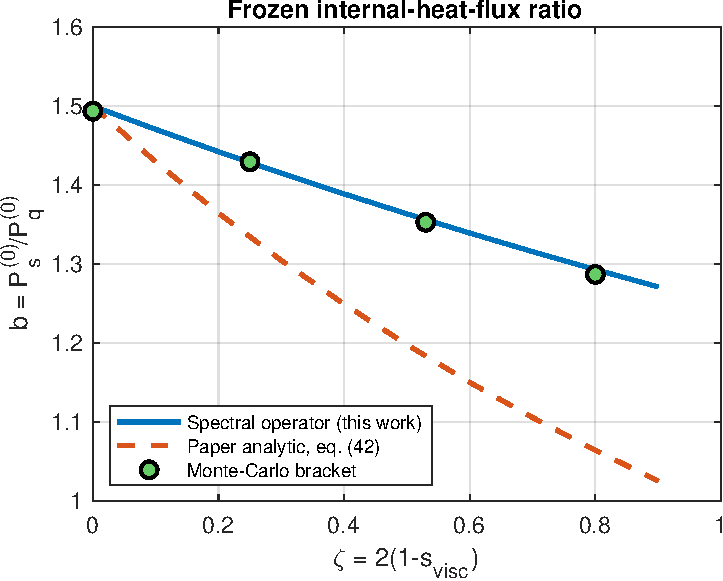
\includegraphics[width=0.62\textwidth]{figures/fig_frozen_pr_bratio.pdf}
\caption{Frozen internal-heat-flux ratio $b=P_s^{(0)}/P_q^{(0)}$ versus the relative-speed
exponent $\zeta$. The spectral operator (solid) tracks the independent Monte-Carlo bracket
(markers); the paper's analytic formula (dashed) deviates with increasing $\zeta$.}
\label{fig:bratio}
\end{figure}

\subsection{Convergence}
The non-frozen channel converges spectrally; the frozen channel converges spectrally after the
$H_\delta$ correction. The internal-energy-modulated extended channels (Sec.~\ref{sec:extended})
couple the velocity and internal energies through the factor $(I/E)^{\hat z}$, whose non-integer
exponent makes a direct product rule converge only algebraically; the auxiliary Laplace integral
of Sec.~\ref{sec:laplace} resolves the coupling and restores spectral convergence
(Fig.~\ref{fig:conv}, quantified in Sec.~\ref{sec:laplaceval}).

\begin{figure}[t]
\centering
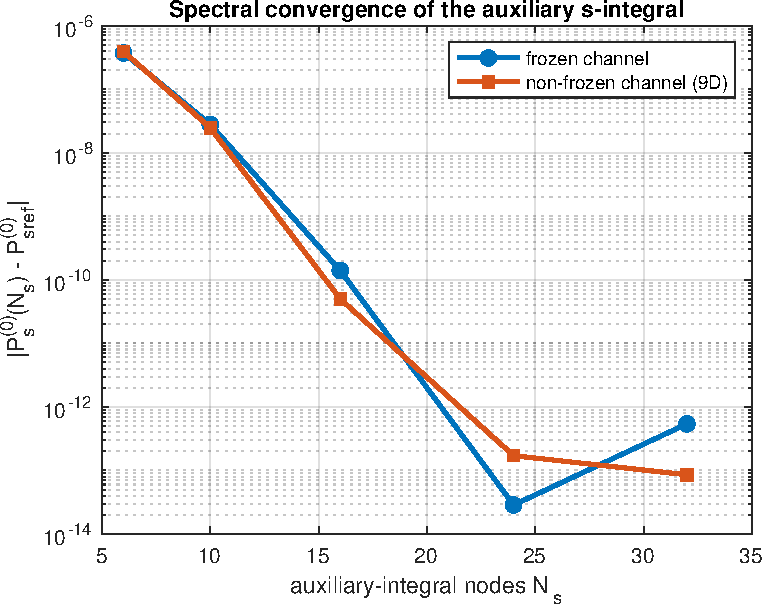
\includegraphics[width=0.62\textwidth]{figures/fig_convergence.pdf}
\caption{Spectral convergence of the auxiliary $s$-integral \eqref{eq:gj}. Error of the production
rate $P_s^{(0)}$ versus the Gauss--Jacobi node count $N_s$, at fixed internal/spatial padding so
that only the $s$-integral error remains. Both the frozen and the 9D non-frozen channel converge
geometrically to machine precision (at essentially the same rate), confirming that the auxiliary
integral resolves the energy coupling $(I/E)^{\hat z}$ in both channels.}
\label{fig:conv}
\end{figure}

\subsection{Transport coefficients of the base model}
Table~\ref{tab:base} lists, for the calorically-perfect gases of \cite[Table~1]{Djordjic2023},
the Eucken and frozen Prandtl numbers and the reachable Prandtl window of the base DSMC model as
$\omega$ ranges over $[0,1]$. With the accurate frozen channel the window is narrow and sits
high: the measured Prandtl numbers fall below it for four of five gases, so the base model
cannot reproduce them -- motivating the extended kernel.

\begin{table}[t]
\centering
\caption{Base DSMC model. Eucken Prandtl number (analytic), our frozen Prandtl number
(Monte-Carlo confirmed), and the reachable $\Pr$ window over $\omega\in[0,1]$, versus the
measured value. ``in/out'' indicates whether the measured value is reachable.}
\label{tab:base}
\begin{tabular}{lccccccc}
\toprule
gas & $\delta$ & $\zeta$ & $\Pr^{\mathrm{Euck}}$ & $\Pr_{\mathrm{frozen}}$ (ours)
    & $\Pr$ window & $\Pr_{\mathrm{meas}}$ & reachable \\
\midrule
\ce{N2} & 2.01 & 0.534 & 0.7371 & 0.7209 & $[0.7209,\,0.7361]$ & 0.717 & out \\
\ce{O2} & 2.07 & 0.442 & 0.7388 & 0.7249 & $[0.7249,\,0.7429]$ & 0.717 & out \\
\ce{NO} & 2.18 & 0.420 & 0.7417 & 0.7280 & $[0.7280,\,0.7467]$ & 0.740 & in  \\
\ce{CO} & 2.01 & 0.530 & 0.7371 & 0.7210 & $[0.7210,\,0.7363]$ & 0.743 & out \\
\ce{H2} & 1.94 & 0.608 & 0.7352 & 0.7173 & $[0.7173,\,0.7305]$ & 0.686 & out \\
\bottomrule
\end{tabular}
\end{table}

% =====================================================================
\section{The internal-energy-modulated extended model}
\label{sec:extended}

\subsection{Kernel and spectral implementation}
The extended model \cite[eq.~(43)]{Djordjic2023} multiplies each channel by an
internal-energy-dependent factor with parameters $(\etah,\zetah)$ (non-frozen) and
$(\etah_f,\zetah_f)$ (frozen):
\begin{equation}
\begin{aligned}
\mathcal{B}=|\uu|^\zeta\Big[\,
& K_\delta\,\omega\,R^{\zeta/2}\big(1+\etah\big[(r(1-R)i)^{\zetah/2}+((1-r)(1-R)i_*)^{\zetah/2}\big]\big) \\
& +\,(1-\omega)\,\delta_{r-r'}\delta_{R-R'}\,e_{\mathrm{tr}}^{\zeta/2}\big(1+\etah_f[i^{\zetah_f}+i_*^{\zetah_f}]\big)\Big],
\end{aligned}
\label{eq:ext}
\end{equation}
with $\etah,\etah_f\ge-\tfrac12$ (kernel positivity) and $\zetah,\zetah_f\ge0$. The negative
$\etah,\etah_f$ allow the internal energy to \emph{lower} the Prandtl number below the
frozen/Eucken curve and to decouple $\nu/\mu$ from $\Pr$. Setting all four parameters to zero
recovers \eqref{eq:dsmc} exactly (verified to $7\times10^{-15}$).

In the sum-factorization cascade the non-frozen factor separates: $(r(1-R))^{\zetah/2}$ splits
into an $r$-weight (inside the partition integral) and a $(1-R)^{\zetah/2}$ weight (at the
kinetic-partition merge), while $i^{\zetah/2}=(I/E)^{\zetah/2}$ is a per-quadrature-point scalar.
Both internal terms weight each post-collision channel, requiring four auxiliary $r$-moments;
the loss term uses the matching integrated moment so that gain and loss share an identical
weighting and conservation is preserved exactly ($\#\text{null}=5$, mass row $\sim5\times10^{-16}$
for $\etah,\etah_f$ of either sign). The frozen factor is a single per-point scalar
$1+\etah_f[(I/E)^{\zetah_f}+(I_*/E)^{\zetah_f}]$ on the elastic weight, which conserves trivially.
Evaluated pointwise on the product Gauss--Laguerre nodes, however, the energy factor
$(I/E)^{\hat z}$ is non-polynomial and the extended channels converge only \emph{algebraically};
Sec.~\ref{sec:laplace} restores spectral convergence by an auxiliary integral.

\subsection{Spectral resolution of the energy coupling via an auxiliary Laplace integral}
\label{sec:laplace}
The factor $i^{\hat z}=(I/E)^{\hat z}$ -- with $\hat z=\zetah/2$ in the non-frozen channel and
$\hat z=\zetah_f$ in the frozen one -- is the only obstruction to spectral convergence of
\eqref{eq:ext}. Written as $i^{\hat z}=I^{\hat z}E^{-\hat z}$, it \emph{couples} the velocity
energy $z=\tfrac12|\uu|^2$ to the internal energies $(I,I_*)$ through $E=z+I+I_*$. These are
independent degrees of freedom carried by the product equilibrium measure
$z^{\zeta/2}e^{-z}\,I^\nu e^{-I}\,I_*^\nu e^{-I_*}$, so the branch point of $E^{-\hat z}$ at
$E\to0$ is \emph{not removable} by any change of the velocity/energy variables -- it merely
relocates -- and a direct product Gauss--Laguerre rule converges only algebraically. We therefore
resolve the coupling by \emph{integration} rather than reparametrization, through the Gamma
(Laplace) representation
\begin{equation}
E^{-\hat z}=\frac{1}{\Gamma(\hat z)}\int_0^\infty s^{\hat z-1}\,e^{-sE}\,ds ,\qquad \hat z>0 .
\label{eq:laplace}
\end{equation}
Because the energy splits \emph{additively with no cross terms}, $E=\tfrac12|\uu|^2+I+I_*$, the
auxiliary exponential factorizes across the three independent axes,
\begin{equation}
e^{-sE}=e^{-s|\uu|^2/2}\;e^{-sI}\;e^{-sI_*},
\label{eq:factorize}
\end{equation}
so that for each fixed $s$ every axis is handled independently on the \emph{unchanged}
sum-factorization machinery of Sec.~\ref{sec:kernel}.

\paragraph{Internal axes.}
The active axis carries both the fractional power $I^{\hat z}$ and the rescaling $e^{-sI}$,
\begin{equation}
\int_0^\infty I^{\nu+\hat z}\,e^{-(1+s)I}\,g(I)\,dI
=\sigma^{\nu+\hat z+1}\!\int_0^\infty \tau^{\nu+\hat z}\,e^{-\tau}\,g(\sigma\tau)\,d\tau,
\qquad \sigma=\frac{1}{1+s},
\label{eq:rescale}
\end{equation}
i.e.\ a Gauss--Laguerre$(\nu+\hat z)$ rule evaluated at \emph{scaled nodes} $\sigma\tau_a$: the
endpoint singularity $I^{\hat z}$ is absorbed into the shifted Laguerre parameter
$\nu\!\to\!\nu+\hat z$ and the Maxwellian rescaling into the node scale $\sigma$. The spectator
axis $I_*$ is identical with $\nu+\hat z\!\to\!\nu$. Both are \emph{spectral} for every $s$, and
$E=\tfrac12|\uu|^2+\sigma\tau_a+\sigma\tau_b$ is reconstructed consistently at the scaled nodes.

\paragraph{Velocity axis.}
The velocity enters \eqref{eq:factorize} only through the entire factor $e^{-s|\uu|^2/2}$, which
adds Gaussian decay and introduces no endpoint singularity. It is therefore applied
\emph{pointwise} on the existing speed-centre-of-mass velocity quadrature (Duffy patches and the
scattering rule), with no change of nodes; the direction stays spectral. This asymmetry -- rescale
the internal nodes, but sample the velocity factor pointwise -- is precisely because the fractional
power $I^{\hat z}$ acts on $I$ alone.

\paragraph{The $s$-integral.}
A plain Gauss--Laguerre$(\hat z-1)$ rule for \eqref{eq:laplace} stalls when the kinetic energy
$c=\tfrac12|\uu|^2$ is small, where the integrand decays slowly as $e^{-cs}$. The substitution
\begin{equation}
t=\frac{s}{1+s}\in[0,1],\qquad
s=\frac{t}{1-t},\quad 1+s=\frac{1}{1-t},\quad ds=\frac{dt}{(1-t)^2},
\label{eq:tsub}
\end{equation}
maps the half-line to the unit interval. Collecting the per-$s$ internal scalings from
\eqref{eq:rescale} (the two inner integrals contribute $\sigma^{\nu+\hat z+1}$ and
$\sigma^{\nu+1}$, hence $\sigma^{2\nu+\hat z+2}=(1-t)^{2\nu+\hat z+2}$) together with
$s^{\hat z-1}\,ds=t^{\hat z-1}(1-t)^{-(\hat z+1)}\,dt$ leaves the canonical Jacobi weight on
$[0,1]$:
\begin{equation}
J_{\mathrm{corr}}
=\frac{1}{\Gamma(\hat z)}\int_0^1 t^{\hat z-1}(1-t)^{2\nu+1}\,\widehat J(t)\,dt
\;\approx\;\frac{1}{\Gamma(\hat z)}\sum_{k=1}^{N_s} w_k\,\widehat J(t_k),
\label{eq:gj}
\end{equation}
where $\{t_k,w_k\}$ is the Gauss--Jacobi$(\alpha{=}2\nu+1,\,\beta{=}\hat z-1)$ rule on $[0,1]$,
with weights normalized to the exact Beta moment $\sum_k w_k=B(\hat z,2\nu+2)$, and $\widehat J(t)$
is one base $R$-tensor build evaluated with the scaled internal nodes of \eqref{eq:rescale} and the
velocity factor $e^{-s|\uu|^2/2}$ of \eqref{eq:factorize} at $s=t/(1-t)$, the $\sigma$-powers
stripped (they are carried by the $(1-t)^{2\nu+1}$ weight). Rule \eqref{eq:gj} is spectral in $t$
uniformly in the kinetic energy.

\paragraph{Channels, post-collision weights, and assembly.}
The two bracket terms in \eqref{eq:ext} give an $I$-channel ($i^{\hat z}$, active axis $I$) and an
$I_*$-channel ($i_*^{\hat z}$, active axis $I_*$), which are summed. In the non-frozen channel the
post-collision prefactor $(r(1-R))^{\hat z}$ (resp.\ $((1-r)(1-R))^{\hat z}$) is bounded and folds
into shifted partition weights -- the kinetic-partition weight gains $(1-R)^{\hat z}$ and the
internal-partition weight gains $r^{\hat z}$ (resp.\ $(1-r)^{\hat z}$); the frozen channel has no
partition integral. Since the operator is linear in $\etah$ (resp.\ $\etah_f$),
\begin{equation}
J(\etah)=J_{\mathrm{base}}+\etah\,J_{\mathrm{corr}},
\end{equation}
the base build is reused unchanged and $J_{\mathrm{corr}}$ is the $\Gamma(\hat z)^{-1}$-weighted
Gauss--Jacobi sum \eqref{eq:gj} of $N_s$ rescaled builds. Because the auxiliary factor multiplies
the gain and loss terms identically, exact conservation is preserved. The extended channels now
converge \emph{spectrally}, replacing the algebraic convergence of the pointwise evaluation.

\subsection{Validation of the spectral path}
\label{sec:laplaceval}
We verify the construction on the production rate $P_s^{(0)}$ (the internal-heat-flux mode,
$\ell{=}1,n{=}1$) at $\delta=2.01$, $\zeta=0.533$, with extended parameters $\hat\eta=\tfrac12$,
$\hat\zeta=0.965$.

\paragraph{Base regression.}
With $\hat\eta=\hat\eta_f=0$ the auxiliary-Laplace path reproduces the base operator built by the
legacy routine to $5.7\times10^{-14}$ (relative $3\times10^{-16}$), for both the frozen
($\omega{=}0$) and non-frozen ($\omega{=}1$) channels: the new path leaves the validated base model
untouched.

\paragraph{Spectral convergence of the $s$-integral.}
The auxiliary integral \eqref{eq:gj} introduces one new quadrature direction, the Gauss--Jacobi
$s$-node count $N_s$. Holding the internal and spatial grids fixed (so their errors are
common-mode and cancel), $P_s^{(0)}$ converges \emph{geometrically} in $N_s$ for both channels
(Fig.~\ref{fig:conv} and Table~\ref{tab:saxis}), reaching machine precision by $N_s\!\approx\!24$.
The frozen and 9D non-frozen channels converge at essentially the same rate, confirming that the
$s$-integral resolves the energy coupling identically in both. A modest $N_s\!\sim\!16$--$24$ is
ample.

\paragraph{Internal direction.}
Once the coupling is resolved, the internal $(I,I_*)$ direction inherits the convergence of the
\emph{base} operator: the elastic frozen channel is converged to machine precision at zero internal
padding (the internal energies are spectators), while the non-frozen channel converges at the base
channel's (geometric) rate. The pointwise evaluation of $(I/E)^{\hat z}$, by contrast, made this
direction merely algebraic -- the defect the auxiliary integral removes.

\begin{table}[t]
\centering
\caption{Spectral convergence of the auxiliary $s$-integral. Error of $P_s^{(0)}$ versus the
Gauss--Jacobi node count $N_s$ at fixed internal/spatial padding (common-mode errors cancelled),
$\delta=2.01$, $\zeta=0.533$, $\hat\eta_{(f)}=\tfrac12$, $\hat\zeta_{(f)}=0.965$. Both channels
converge geometrically to machine precision.}
\label{tab:saxis}
\begin{tabular}{cccccc}
\toprule
$N_s$ & $6$ & $10$ & $16$ & $24$ & $32$ \\
\midrule
frozen            & $3.7\times10^{-7}$ & $2.8\times10^{-8}$ & $1.4\times10^{-10}$ & $2.9\times10^{-14}$ & --- \\
non-frozen (9D)   & $3.9\times10^{-7}$ & $2.5\times10^{-8}$ & $5.0\times10^{-11}$ & $1.7\times10^{-13}$ & $8.5\times10^{-14}$ \\
\bottomrule
\end{tabular}
\end{table}

\subsection{Reaching the experimental Prandtl number and bulk/shear ratio}
Following \cite{Djordjic2023} we fix $(\etah,\zetah)$ and re-fit the remaining parameters to the
measured $\Pr$ (Table~2 of \cite{Djordjic2023}) and $\nu/\mu$ (Table~3). Because the operator is
\emph{linear} in $\etah_f$, the convex blend
$J(\omega,\etah_f)=\omega J_{\mathrm{nf}}+(1-\omega)(J_{\mathrm{fr}}^{0}+\etah_f J_{\mathrm{fr}}^{\eta})$
is formed from three pre-built operators, making the $(\omega,\etah_f)$ solve a fast $2\times2$
root-find. Table~\ref{tab:ext} reports, for each gas: the measured pair; the values our operator
returns at the paper's Table-4 parameters (close but not exact, as expected from
Sec.~\ref{sec:frozenpr}); and our re-fit, which reaches the experimental $\Pr$ and $\nu/\mu$
simultaneously. For \ce{H2} the extreme bulk/shear ratio forces $\omega\!\approx\!0.01$, where
$\etah$ has no leverage, so the frozen exponent $\zetah_f$ is freed as well.
Figure~\ref{fig:reach} visualizes the result.

\begin{table}[t]
\centering
\caption{Extended model. Measured transport pair vs.\ our operator at the paper's Table-4
parameters (E3) and after re-fitting in our operator (E4). For \ce{N2} and \ce{CO} the re-fit
reaches the experimental $\Pr$ and $\nu/\mu$ \emph{exactly} with admissible parameters
($\etah_f\ge-\tfrac12$). For \ce{H2} the experimental point is hit exactly only at
$\etah_f\approx-0.506$, i.e.\ marginally ($0.006$) beyond the strict positivity bound -- our
accurate operator places \ce{H2} essentially \emph{on} the model's positivity boundary (the
documented extreme gas, whose measured $\Pr$ lies below the frozen curve).}
\label{tab:ext}
\begin{tabular}{lcc cc ccc}
\toprule
& \multicolumn{2}{c}{measured} & \multicolumn{2}{c}{E3: Table-4 params}
& \multicolumn{3}{c}{E4: re-fit (this work)} \\
\cmidrule(lr){2-3}\cmidrule(lr){4-5}\cmidrule(lr){6-8}
gas & $\Pr$ & $\nu/\mu$ & $\Pr$ & $\nu/\mu$ & $\Pr$ & $\nu/\mu$ & $(\omega,\etah_f,\zetah_f)$ \\
\midrule
\ce{N2} & 0.717 & 0.73 & 0.7188 & 0.8532 & 0.7170 & 0.7300 & $(0.342,-0.263,0.300)$ \\
\ce{CO} & 0.743 & 0.55 & 0.7413 & 0.6343 & 0.7430 & 0.5500 & $(0.606,\;0.687,0.965)$ \\
\ce{H2} & 0.686 & 30.0 & 0.7116 & 36.10  & 0.6860 & 30.00  & $(0.001,-0.504,0.050)^{\dagger}$ \\
\bottomrule
\end{tabular}

\smallskip
{\footnotesize $^{\dagger}$\,$\etah$ fixed at the Table-4 value $-0.453$; the experimental point is
hit exactly (residual $10^{-11}$) at $\etah_f=-0.504$, only $0.004$ below the strict positivity
bound $-\tfrac12$.}
\end{table}

\begin{figure}[t]
\centering
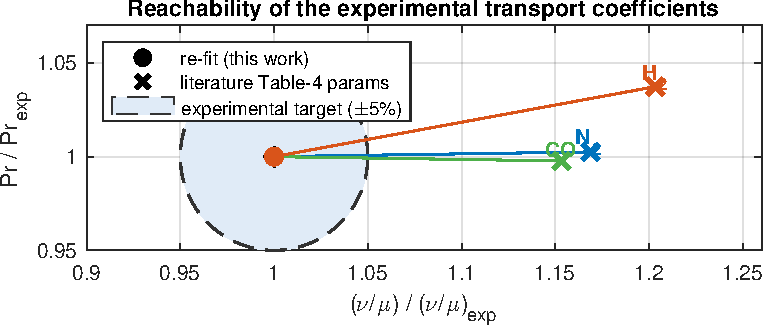
\includegraphics[width=0.72\textwidth]{figures/fig_reachability.pdf}
\caption{Reachability of the experimental transport coefficients, in coordinates normalized to each
gas's measured values so every target collapses to $(1,1)$ -- a true relative-tolerance circle is
then meaningful despite $\nu/\mu$ ranging from $\sim\!0.6$ (\ce{N2},\ce{CO}) to $\sim\!30$
(\ce{H2}). Crosses are the operator at the paper's Table-4 parameters (E3): they miss, overshooting
$\nu/\mu$ by $15$--$20\%$. Filled dots are our re-fit (E4): every gas lands inside the experimental
target (shaded, a $\pm5\%$ guide), matching the measured $\Pr$ and $\nu/\mu$ \emph{simultaneously}.
Colours distinguish the gases; the line traces the re-fit displacement.}
\label{fig:reach}
\end{figure}

% =====================================================================
\section{Conclusions}
\label{sec:conclusions}

We integrated the DSMC VHS--Borgnakke--Larsen kernel and its internal-energy-modulated extension
into a spectral Wigner--Eckart evaluation of the polyatomic Boltzmann collision operator. The key
methodological point is the correct spectral treatment of the frozen channel (no
$(R,r)$-partition measure), without which the internal heat-flux relaxation acquires a spurious
$\delta$-dependence. The corrected operator meets the Eucken and shear anchors exactly, and an
independent Monte-Carlo bracket shows that the spectral frozen Prandtl number is more accurate
than the paper's analytic formula at hard-potential exponents. The extended kernel, re-fitted in
our operator, reaches the experimental Prandtl number and bulk/shear viscosity ratio
simultaneously for \ce{N2} and \ce{CO} with admissible parameters, and for the extreme case
\ce{H2} exactly but at the kernel-positivity boundary ($\etah_f=-0.504$, $0.004$ below
$-\tfrac12$) -- consistent with \ce{H2} lying below the frozen Prandtl curve.

\section*{Reproducibility}
The kernel is exposed through \code{ScatteringKernel('DSMC',\,struct(...))}; the base and extended
models are assembled by \code{GeneralCollisionTensor.generate\_R\_tensor\_sumfac} and the MEX
routine \code{compute\_rtensor\_polyatomic\_sumfac\_mex} (channels \code{kernel\_model=1} non-frozen,
\code{2} frozen). The base transport table (Table~\ref{tab:base}) is produced by
\code{benchmark\_dsmc\_transport.m}; the extended-model results (Table~\ref{tab:ext}) by
\code{benchmark\_dsmc\_extended.m}; and the figures by \code{paper/make\_figures.m}. See the
repository \code{README.md} for the DSMC/extended kernel usage and the MEX build recipe.

\begin{thebibliography}{9}
\bibitem{Djordjic2023}
V.~Djordji\'c, G.~Oblapenko, M.~Pavi\'c-\v{C}oli\'c, M.~Torrilhon,
\emph{Boltzmann collision operator for polyatomic gases in agreement with experimental data and
DSMC method}, Continuum Mech.\ Thermodyn.\ \textbf{35} (2023) 103--119.
\end{thebibliography}

\end{document}
